
%%%%%%%%%%%%%%%%%%%%%%%%%%%%%%%%%%%%%%%%%%%%%%%%%%%%%%%%
\documentclass[12pt,a4paper]{article}% 文档格式
\usepackage{ctex,hyperref}% 输出汉字
\usepackage{times}% 英文使用Times New Roman
%%%%%%%%%%%%%%%%%%%%%%%%%%%%%%%%%%%%%%%%%%%%%%%%%%%%%%%%
\title{\fontsize{18pt}{27pt}\selectfont% 小四字号,1.5倍行距
	{\heiti% 黑体 
		Physics Homework}}% 题目
%%%%%%%%%%%%%%%%%%%%%%%%%%%%%%%%%%%%%%%%%%%%%%%%%%%%%%%%
\author{\fontsize{12pt}{18pt}\selectfont% 小四字号,1.5倍行距
	{\fangsong% 仿宋
		Haixuan Lin}\\% 标题栏脚注
	\fontsize{10.5pt}{15.75pt}\selectfont% 五号字号,1.5倍行距
	{\fangsong% 仿宋
		(Fudan University department of physics
		)}}% 作者单位,“~”表示空格
%%%%%%%%%%%%%%%%%%%%%%%%%%%%%%%%%%%%%%%%%%%%%%%%%%%%%%%%
\date{}% 日期(这里避免生成日期)
%%%%%%%%%%%%%%%%%%%%%%%%%%%%%%%%%%%%%%%%%%%%%%%%%%%%%%%%
\usepackage{amsmath,amsfonts,amssymb}% 为公式输入创造条件的宏包
%%%%%%%%%%%%%%%%%%%%%%%%%%%%%%%%%%%%%%%%%%%%%%%%%%%%%%%%
\usepackage{graphicx}% 图片插入宏包
\usepackage{subfigure}% 并排子图
\usepackage{float}% 浮动环境,用于调整图片位置
\usepackage[export]{adjustbox}% 防止过宽的图片
\usepackage{pdfpages}
%%%%%%%%%%%%%%%%%%%%%%%%%%%%%%%%%%%%%%%%%%%%%%%%%%%%%%%%
\usepackage{bibentry}
\usepackage{natbib}% 以上2个为参考文献宏包
%%%%%%%%%%%%%%%%%%%%%%%%%%%%%%%%%%%%%%%%%%%%%%%%%%%%%%%%
\usepackage{abstract}% 两栏文档,一栏摘要及关键字宏包
\renewcommand{\abstracttextfont}{\fangsong}% 摘要内容字体为仿宋
\renewcommand{\abstractname}{\textbf{摘\quad 要}}% 更改摘要二字的样式
%%%%%%%%%%%%%%%%%%%%%%%%%%%%%%%%%%%%%%%%%%%%%%%%%%%%%%%%
\usepackage{xcolor}% 字体颜色宏包
\newcommand{\red}[1]{\textcolor[rgb]{1.00,0.00,0.00}{#1}}
\newcommand{\blue}[1]{\textcolor[rgb]{0.00,0.00,1.00}{#1}}
\newcommand{\green}[1]{\textcolor[rgb]{0.00,1.00,0.00}{#1}}
\newcommand{\darkblue}[1]
{\textcolor[rgb]{0.00,0.00,0.50}{#1}}
\newcommand{\darkgreen}[1]
{\textcolor[rgb]{0.00,0.37,0.00}{#1}}
\newcommand{\darkred}[1]{\textcolor[rgb]{0.60,0.00,0.00}{#1}}
\newcommand{\brown}[1]{\textcolor[rgb]{0.50,0.30,0.00}{#1}}
\newcommand{\purple}[1]{\textcolor[rgb]{0.50,0.00,0.50}{#1}}% 为使用方便而编辑的新指令
%%%%%%%%%%%%%%%%%%%%%%%%%%%%%%%%%%%%%%%%%%%%%%%%%%%%%%%%
\usepackage{url}% 超链接
\usepackage{bm}% 加粗部分公式
\usepackage{multirow}
\usepackage{booktabs}
\usepackage{epstopdf}
\usepackage{epsfig}
\usepackage{longtable}% 长表格
\usepackage{supertabular}% 跨页表格
\usepackage{algorithm}
\usepackage{algorithmic}
\usepackage{changepage}% 换页
%%%%%%%%%%%%%%%%%%%%%%%%%%%%%%%%%%%%%%%%%%%%%%%%%%%%%%%%
\usepackage{enumerate}% 短编号
\usepackage{caption}% 设置标题
\captionsetup[figure]{name=\fontsize{10pt}{15pt}\selectfont Figure}% 设置图片编号头
\captionsetup[table]{name=\fontsize{10pt}{15pt}\selectfont Table}% 设置表格编号头
%%%%%%%%%%%%%%%%%%%%%%%%%%%%%%%%%%%%%%%%%%%%%%%%%%%%%%%%
\usepackage{indentfirst}% 中文首行缩进
\usepackage[left=2.50cm,right=2.50cm,top=2.80cm,bottom=2.50cm]{geometry}% 页边距设置
\renewcommand{\baselinestretch}{1.5}% 定义行间距(1.5)
%%%%%%%%%%%%%%%%%%%%%%%%%%%%%%%%%%%%%%%%%%%%%%%%%%%%%%%%
\usepackage{fancyhdr} %设置全文页眉、页脚的格式
\pagestyle{fancy}
\hypersetup{colorlinks=true,linkcolor=black}% 去除引用红框,改变颜色
%%%%%%%%%%%%%%%%%%%%%%%%%%%%%%%%%%%%%%%%%%%%%%%%%%%%%%%%
\usepackage{caption}%标题取消自动figure
\usepackage{multicol}
\usepackage{cuted}
%%%%%%%%%%%%%%%%%%%%%%%%%%%%%%%%%%%%%%%%%%%%%%%%%%%%%%%%
\begin{document}% 以下为正文内容
	\maketitle% 产生标题,没有它无法显示标题
	%%%%%%%%%%%%%%%%%%%%%%%%%%%%%%%%%%%%%%%%%%%%%%%%%%%%%%%%
	\lhead{}% 页眉左边设为空
	\chead{}% 页眉中间设为空
	\rhead{}% 页眉右边设为空
	\lfoot{}% 页脚左边设为空
	\cfoot{\thepage}% 页脚中间显示页码
	\rfoot{}% 页脚右边设为空
	%%%%%%%%%%%%%%%%%%%%%%%%%%%%%%%%%%%%%%%%%%%%%%%%%%%%%%%%
	
	
		\begin{center}% 居中处理
			{\textbf{Abstract}}% 英文摘要
		\end{center}
		\begin{adjustwidth}{1.06cm}{1.06cm}% 英文摘要内容
			\hspace{1.5em}In order to improve my computer and English skills, please allow me to complete this physics homework in English context with \LaTeX, so as to improve my professional level. Sorry for the inconvenience!
		\end{adjustwidth}
	
	
	
	\newpage% 从新的一页继续
	
	
	
	\section{Question 6-3}
	\noindent Define $M$ as the mass of the complete big disc. So
	\begin{equation}
		\frac{m}{1}=\frac{M}{1-3\times\frac{1}{9}}
	\end{equation}
	The moment of inertia of the complete disk is
	\begin{equation}
		J_0=\frac{1}{2}MR^2
	\end{equation}
	According to the parallel-axis theorem, the moment of inertia of each cut small disk is
	\begin{equation}
		J_i=\frac{1}{2}\frac{M}{9}\left(\frac{R}{3}\right)^2+\frac{M}{9}\left(\frac{R}{2}\right)^2
	\end{equation}
	As a result
	$$
	J=J_0-3J_i=\frac{43}{72}mR^2
	$$
	
	\section{Question 6-8}
	\subsection*{(1)}
	\noindent Take any thin ring element in the upper disk
	\begin{equation}
		\mathrm{d}m=\frac{3m}{\pi R^2}\cdot2\pi r \mathrm{d}r
	\end{equation}
	Do force analysis of this element
	\begin{equation}
		\mathrm{d}f=\mu \mathrm{d}mg
	\end{equation}
	\begin{equation}
		\mathrm{d}M_f=r\mathrm{d}f
	\end{equation}
	So
	\begin{equation}
		M=\int_0^R{6\mu mg\frac{r^2}{R^2}\mathrm{d}r}=2\mu mgR
	\end{equation}
	The discs both above and below has own moment of inertia
	\begin{equation}
		J_1=\frac{1}{2}3mR^2
	\end{equation}
	\begin{equation}
		J_2=\frac{1}{2}mR^2
	\end{equation}
	According to rotation law
	\begin{equation}
		\beta _1=\frac{M}{J_1}
	\end{equation}
	\begin{equation}
		\beta _2=\frac{M}{J_2}
	\end{equation}
	As a result
	\begin{equation*}
		\Delta t=\frac{\omega_0}{\beta_1+\beta_2}=\frac{3}{16}\frac{R\omega_0}{\mu g}
	\end{equation*}
	\subsection*{(2)}
	\noindent According to kinematic formula of angle
	\begin{equation*}
		\omega=\omega_0-\beta_1\Delta t=\frac{3}{4}\omega_0
	\end{equation*}
	
	\section{Question 6-9}
	\subsection*{(1)}
	\begin{figure}[H]
		\centering
		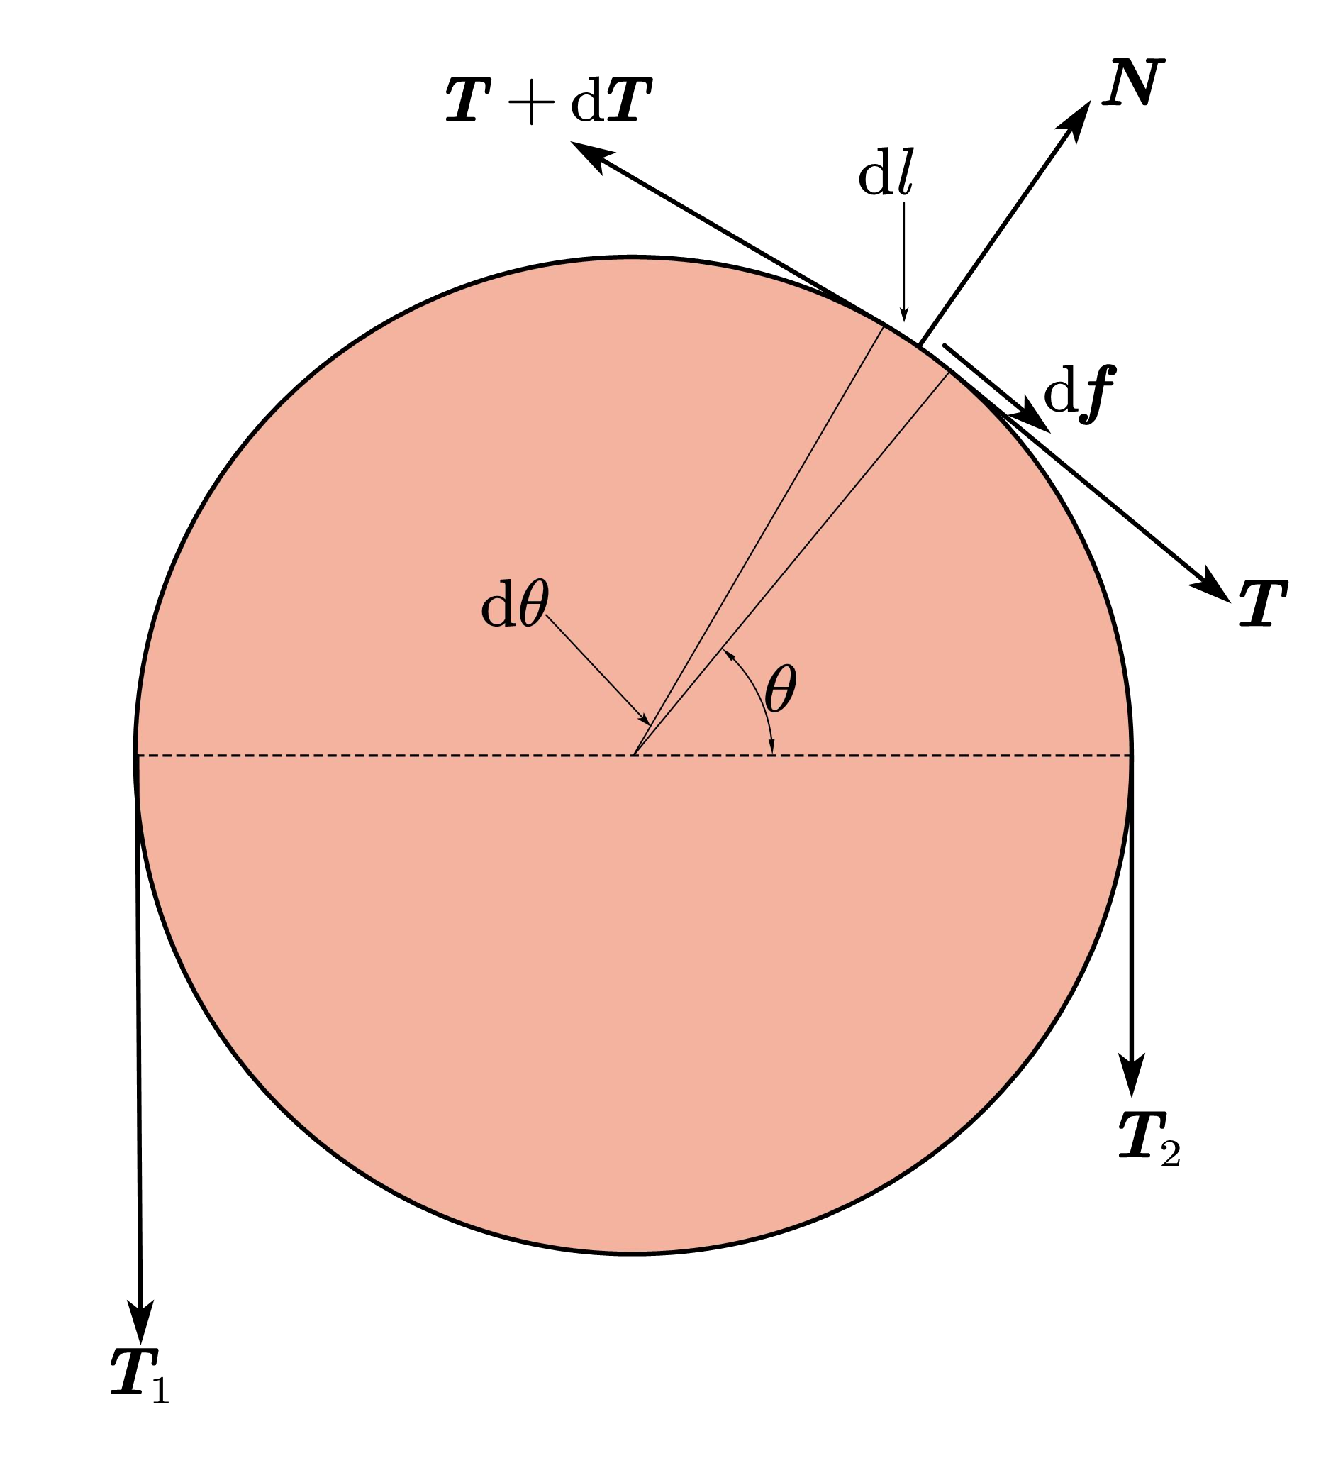
\includegraphics[width=0.7\linewidth]{ATWD}
		\caption*{}
		\label{fig:atwd}
	\end{figure}
	\noindent Take a tiny element of the rope above the Atwood machine to analyse.
	\begin{equation}
		\mathrm{d}N=T\mathrm{d}\theta 
	\end{equation}
	\begin{equation}
		\mathrm{d}f=\mu \mathrm{d}N=\mu T\mathrm{d}\theta 
	\end{equation}
	Combine these two equations and we get a differential equation
	\begin{equation}
		\frac{\mathrm{d}T}{T}=\mu \mathrm{d}\theta 
	\end{equation}
	The solution is that
	\begin{equation}
		T=T_2\mathrm{e}^{\mu \theta}
	\end{equation}
	Further have
	\begin{equation}
		f=\int_0^{\pi}{\mu T_2\mathrm{e}^{\mu \theta}\mathrm{d}\theta}=T_2(\mathrm{e}^{\mu\pi}-1)
	\end{equation}
	The system consists of $m_1$ and $m_2$ and the rope has the same acceleration with the part of only $m_2$. So according to the Newton's second law
	\begin{equation}
		\frac{\left( m_1-m_2 \right) g-f}{m_1+m_2}=\frac{T_2}{m_2}-g=a
	\end{equation}
	So the solution is that
	\begin{equation*}
		a=\frac{m_1-m_2\mathrm{e}^{\mu\pi}}{m_1+m_2\mathrm{e}^{\mu\pi}}g
	\end{equation*}
	\subsection*{(2)}
	\noindent The moment of inertia of the Atwood machine is
	\begin{equation}
		J=\frac{1}{2}mR^2
	\end{equation}
	So according to the law of rotation
	\begin{equation*}
		\alpha=\frac{Rf}{J}=\frac{4m_1m_2g(\mathrm{e}^{\mu\pi}-1)}{mR(m_1+m_2\mathrm{e}^{\mu\pi})}
	\end{equation*}
	\section{Question 6-12}
	\subsection*{(1)}
	\noindent As the figure below, the moment of force $\boldsymbol{N}_\mathrm{A}$ and $\boldsymbol{F}_\mathrm{c}$ of the above half are equivalent.
	\begin{figure}[H]
		\begin{minipage}{0.45\textwidth}
			\centering
			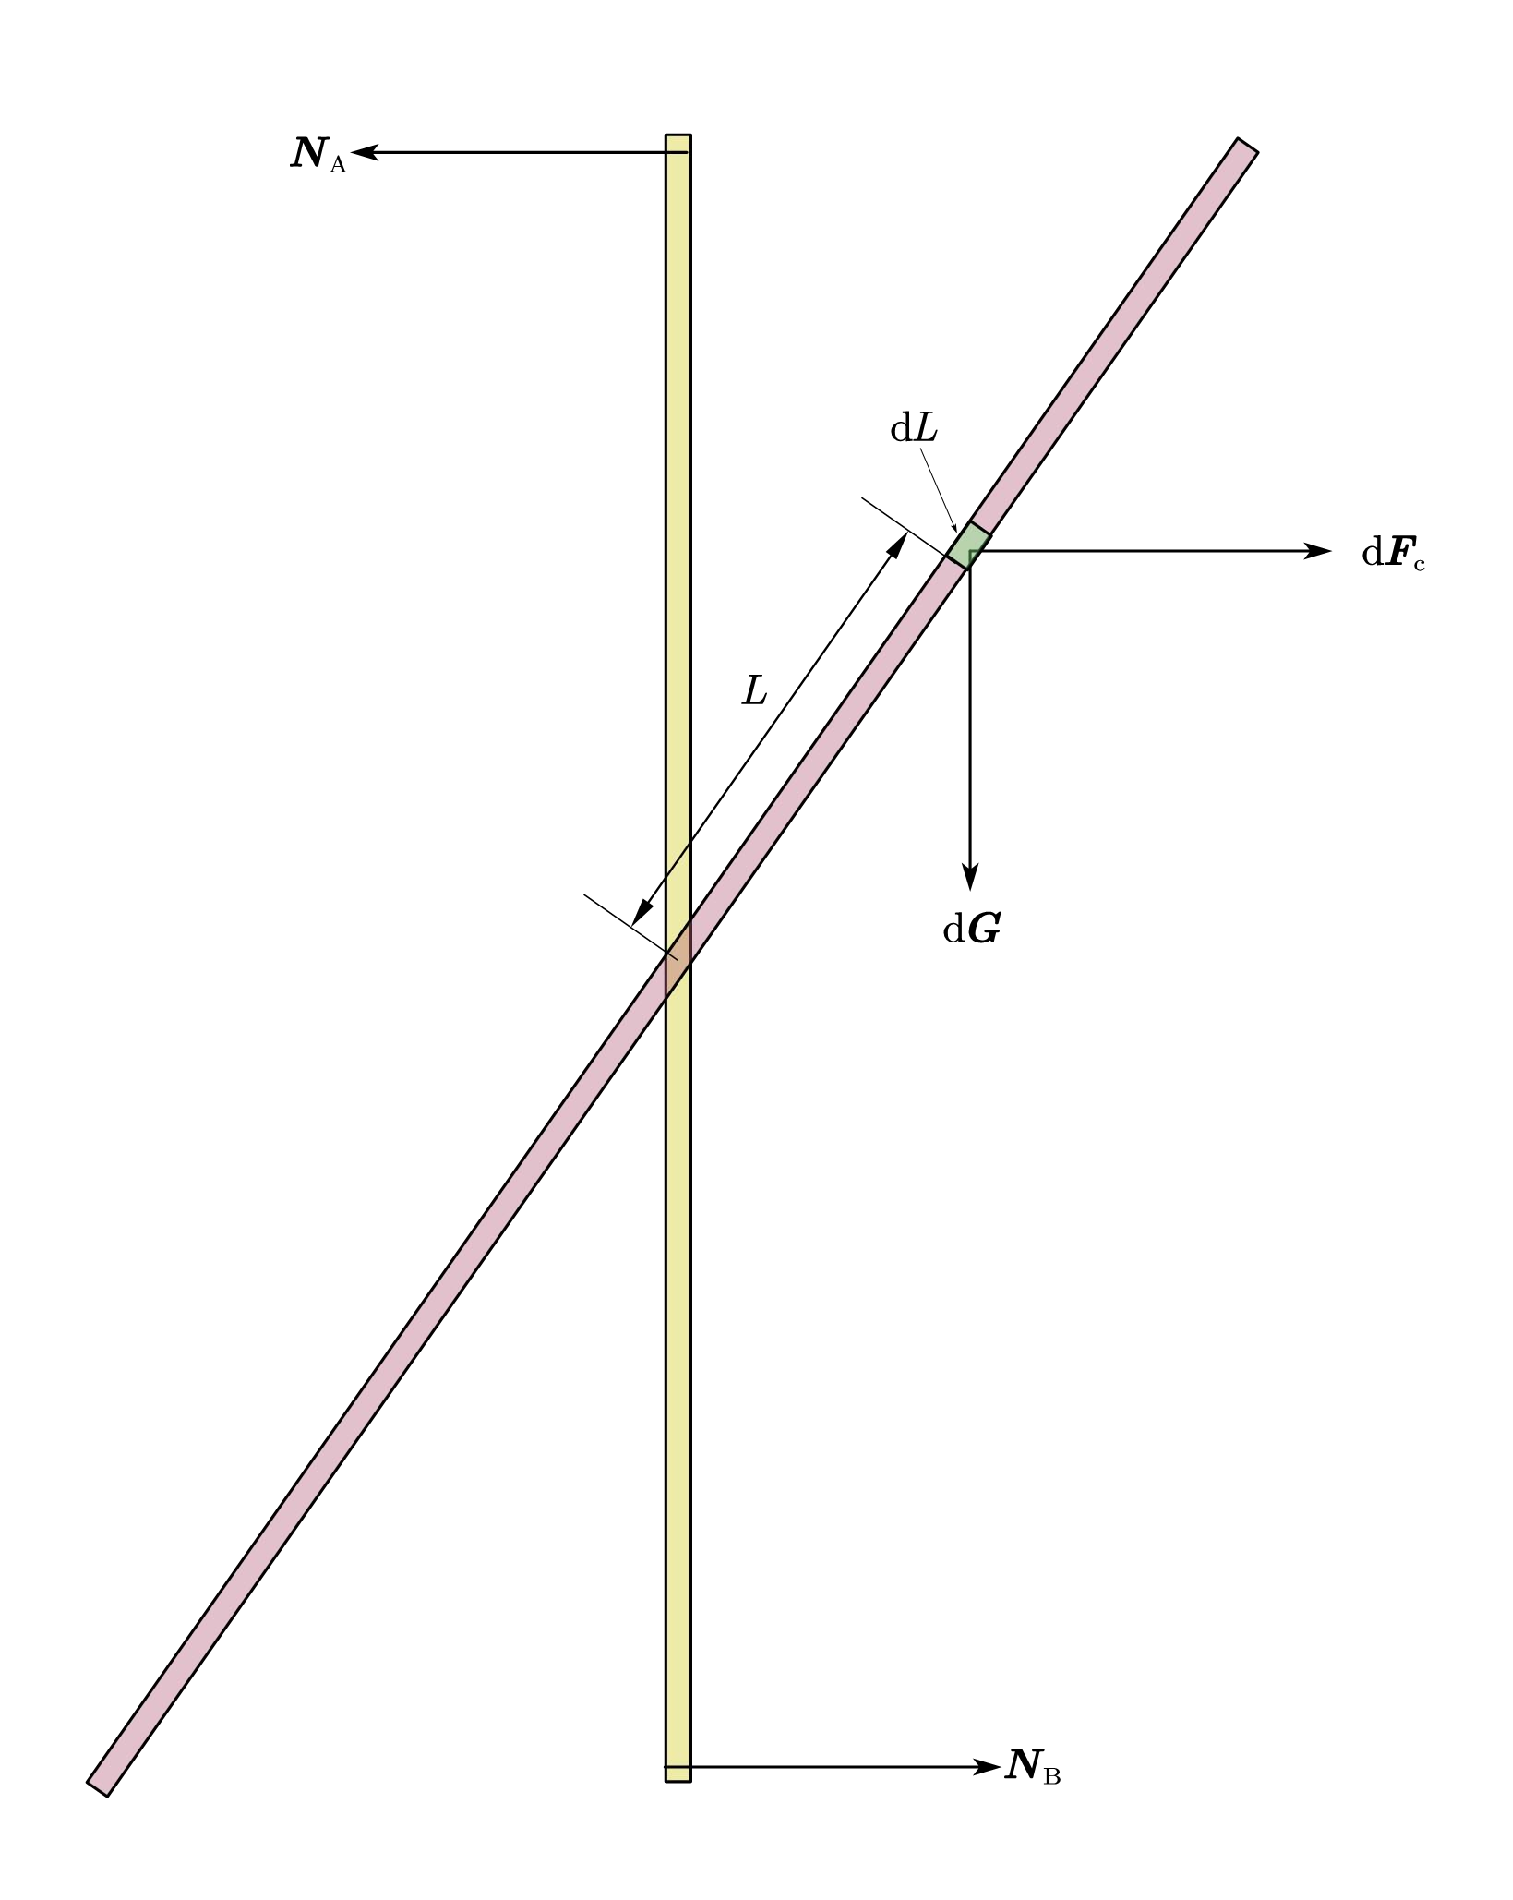
\includegraphics[width=\linewidth]{6-12}
			\caption*{}
		\end{minipage}
		\hfill
		\begin{minipage}{0.45\textwidth}
			\centering
			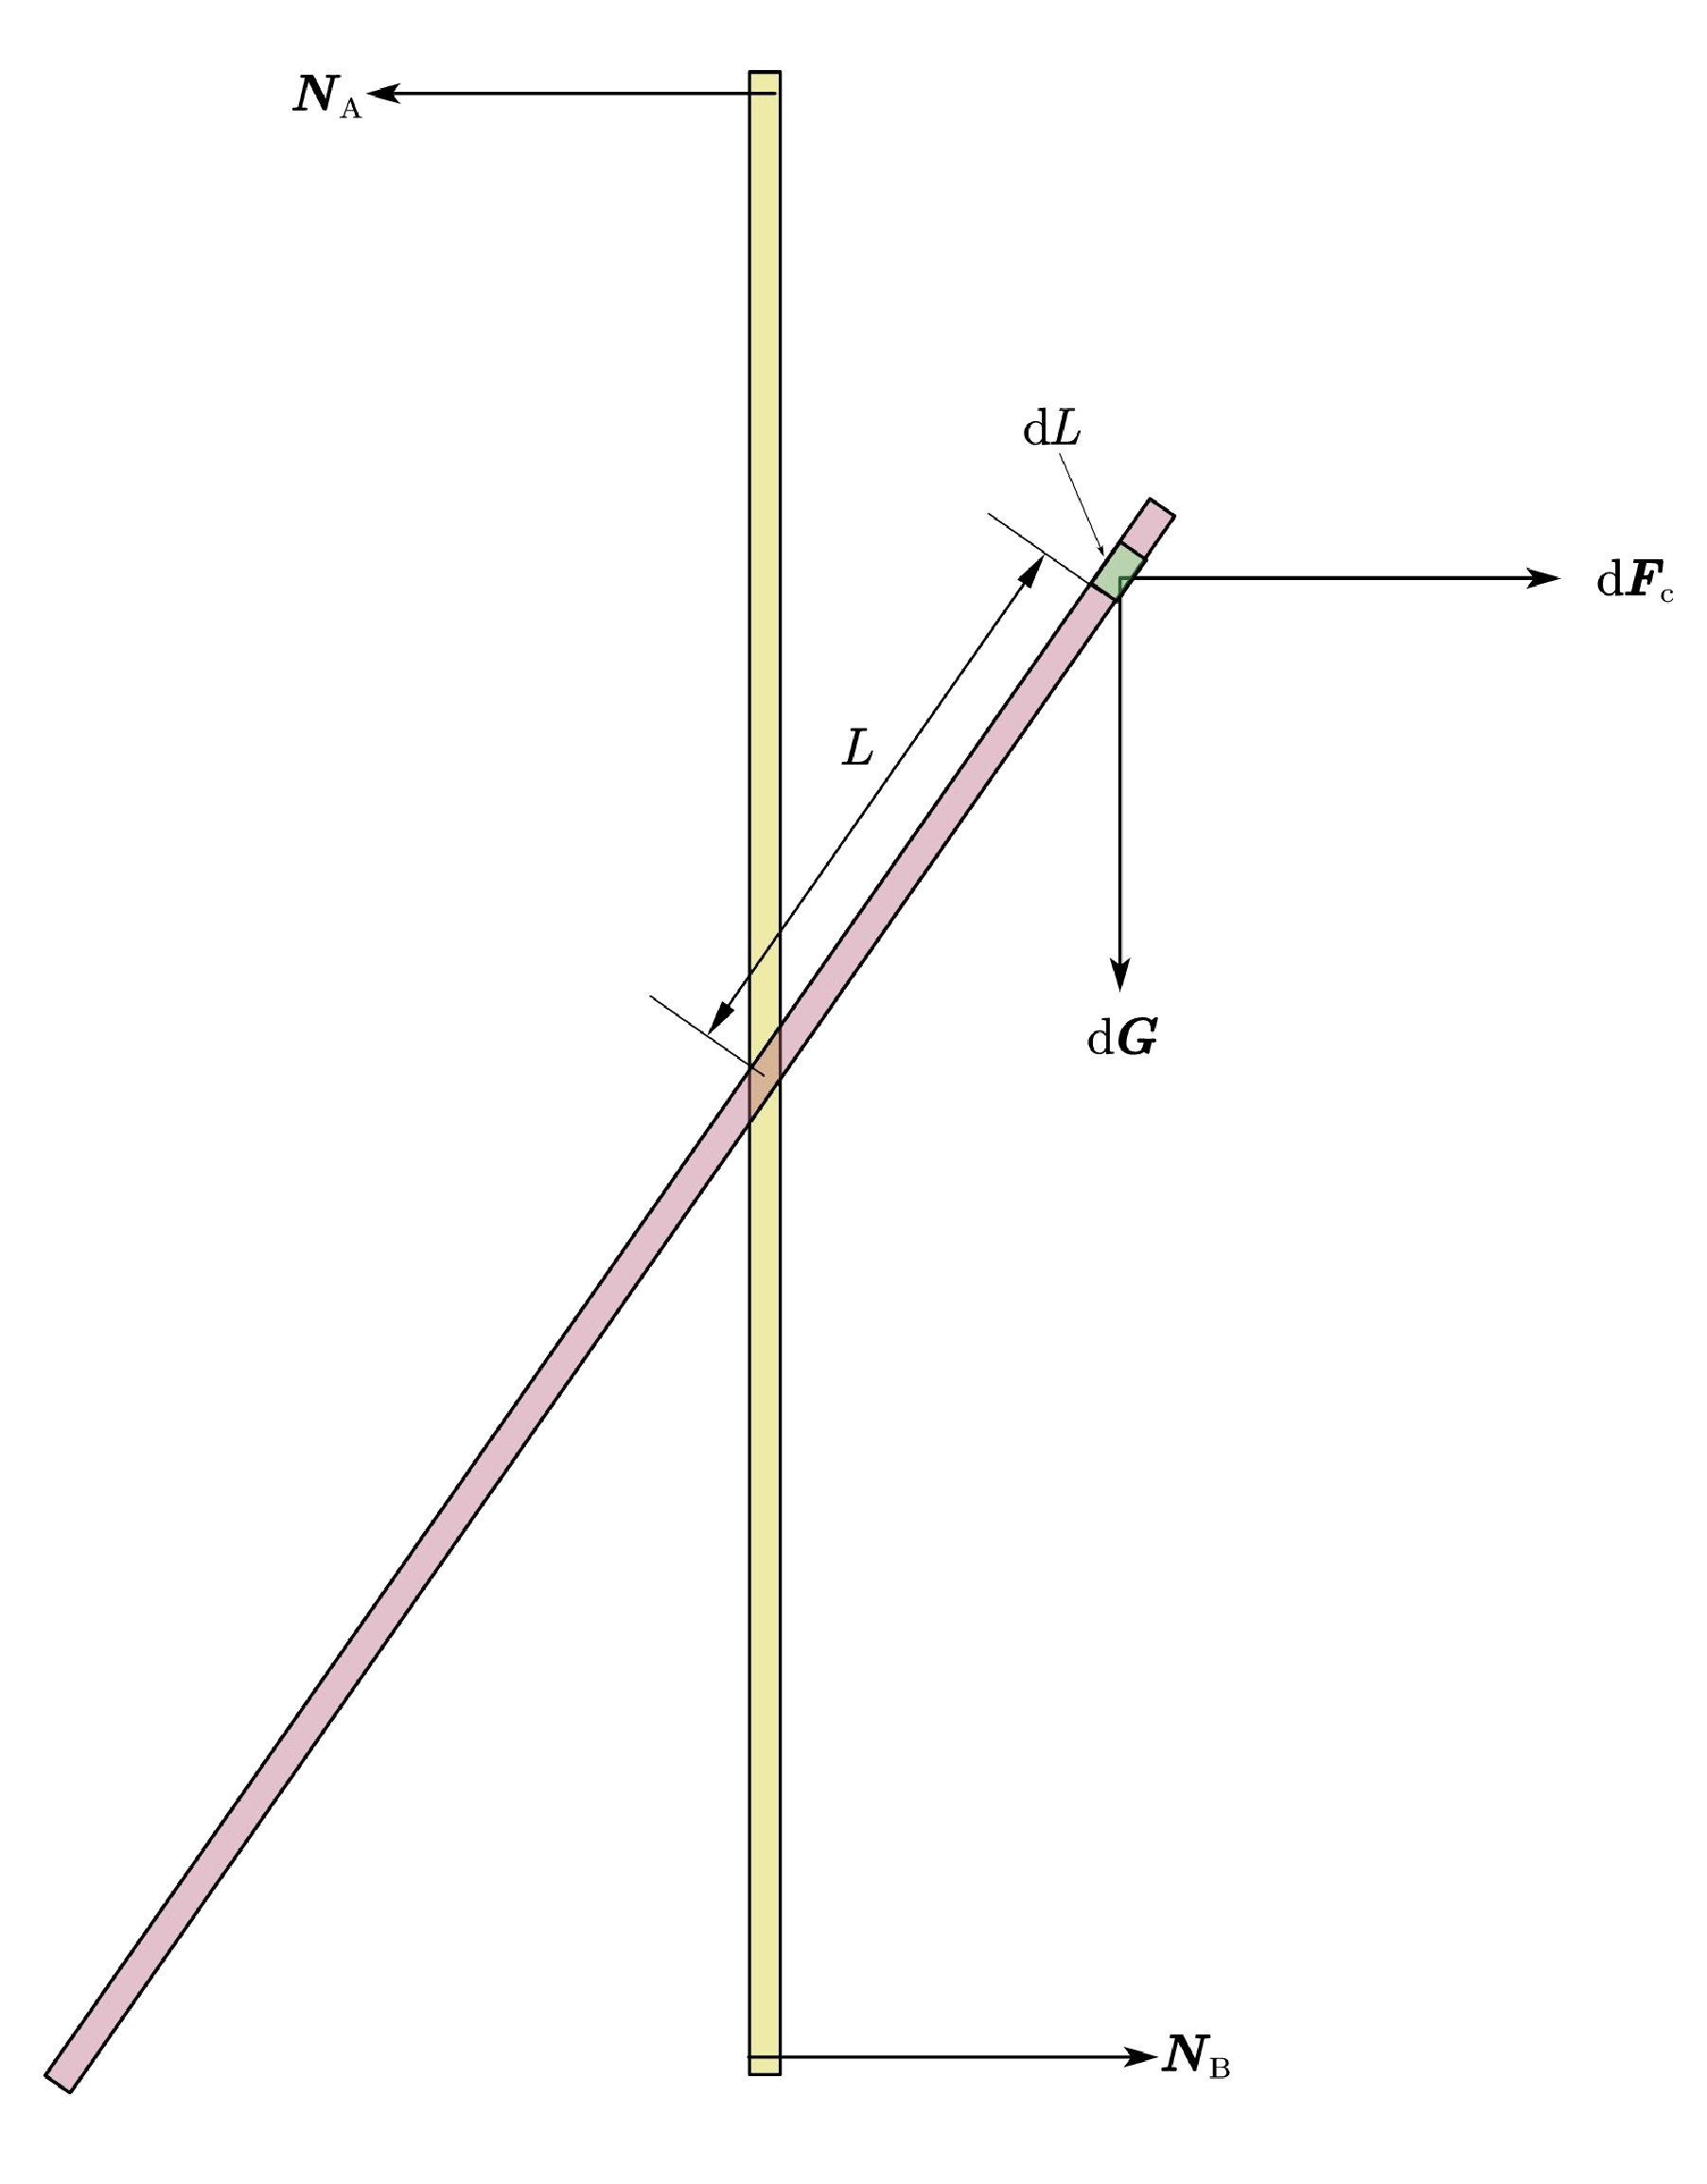
\includegraphics[width=\linewidth]{6-12-2}
			\caption*{}
		\end{minipage}
	\end{figure}
	\begin{equation}
		N_\mathrm{A}R=\int_0^{\frac{1}{2}l}{\frac{\mathrm{d}L}{l}m}\omega ^2L\cos \theta L\sin \theta 
	\end{equation}
	And according to the symmetry, $\boldsymbol{N}_\mathrm{A}=-\boldsymbol{N}_\mathrm{B}$, so
	\begin{equation*}
		N_\mathrm{A}=N_\mathrm{B}=\frac{1}{24R}m\omega ^2l^2\sin \theta \cos \theta 
	\end{equation*}
	\subsection*{(2)}
	\noindent The basic idea doesn't change, but because of the broken symmetry, we have to consider the torque of gravity.
	\begin{equation}
		\mathrm{d}G=\frac{\mathrm{d}L}{l}mg
	\end{equation}
	\begin{equation}
		\mathrm{d}M_{\mathrm{G}}=L\sin \theta \cdot \mathrm{d}G=L\sin \theta \cdot \frac{\mathrm{d}L}{l}mg
	\end{equation}
	Get by integrating.
	\begin{equation}
		M_{\mathrm{G}}=\int \mathrm{d}M_\mathrm{G}=\frac{mg\sin \theta}{l}\int_{\frac{1}{4}l}^{\frac{1}{2}l}{L\mathrm{d}L}
		=\frac{3}{32}mg\sin \theta
	\end{equation}
	
	\noindent Now consider centrifugal force.
	\begin{equation}
		\mathrm{d}F_{\mathrm{c}}=\frac{\mathrm{d}L}{l}m\omega ^2L\sin \theta 
		\mathrm{d}M_{\mathrm{c}}=L\cos \theta \mathrm{d}F_{\mathrm{c}}
		=\frac{\mathrm{d}L}{l}m\omega ^2L^2\sin \theta \cos \theta
	\end{equation}
	Get by integrating.
	\begin{equation}
		F_{\mathrm{c}}=\int_{\frac{1}{4}l}^{\frac{1}{2}l}{\frac{\mathrm{d}L}{l}m\omega ^2L\sin \theta} =\frac{3}{32}m\omega ^2L\sin \theta 
	\end{equation}	 
	\begin{equation}
		M_{\mathrm{c}}=\int_{\frac{1}{4}l}^{\frac{1}{2}l}{\frac{\mathrm{d}L}{l}m\omega ^2L^2\sin \theta \cos \theta} =\frac{3}{64}m\omega ^2l^2\sin \theta \cos \theta			
	\end{equation}
	According to the equations of mechanical equilibrium we have
	\begin{equation}
		\left( N_{\mathrm{A}}+N_{\mathrm{B}} \right) R=M_{\mathrm{c}}-M_{\mathrm{G}}
	\end{equation}
	\begin{equation}
		N_{\mathrm{B}}-N_{\mathrm{A}}=F_{\mathrm{c}}
	\end{equation}
	The solution is that
	\begin{equation*}
		N_{\mathrm{A}}=\frac{3}{128}ml\sin \theta \left[ \frac{1}{R}\left( l\omega ^2\cos \theta -2g \right) -2\omega ^2 \right] 
	\end{equation*}
	\begin{equation*}
		N_B=\frac{3}{128}ml\sin \theta \left[ \frac{1}{R}\left( l\omega ^2\cos \theta -2g \right) +2\omega ^2 \right] 
	\end{equation*}
	\section{Question 6-19}
	\begin{figure}[H]
		\centering
		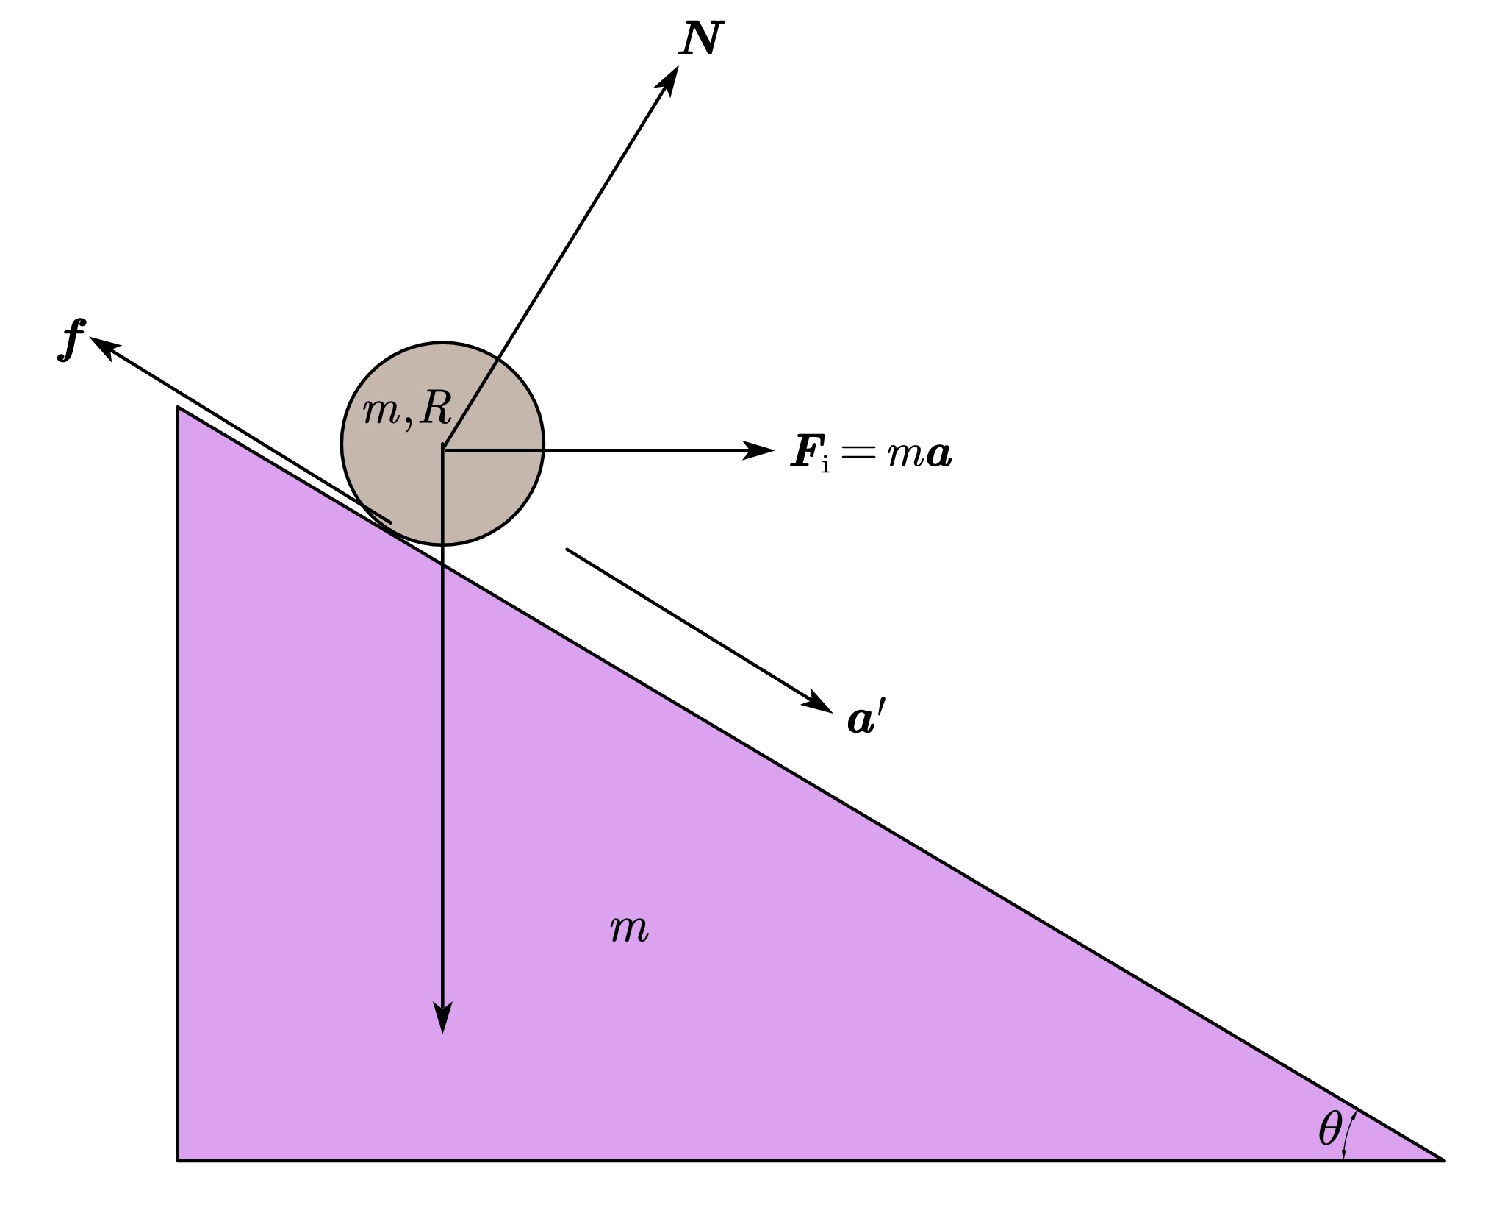
\includegraphics[width=0.7\linewidth]{6-19}
		\caption*{}
		\label{fig:6-19}
	\end{figure}
	\noindent Taking the slope as the reference frame, the force of the cylinder is considered, and the inertia force $\boldsymbol{F}_\mathrm{i}$ is corrected. According to the Newton's second law
	\begin{equation}
		ma'=mg\sin \theta +ma\cos \theta -f
	\end{equation}
	\begin{equation}
		mg\cos\theta=N+ma\sin\theta
	\end{equation}
	Because it is rolling without slipping, the axis of rotation is tangent to the cylinder and the bevel
	, according to the law of rotation and parallel-axis theorem
	\begin{equation}
		mgR\sin \theta +maR\cos \theta 
		=\left( \frac{1}{2}mR^2+mR^2 \right) \beta
		=\left( \frac{1}{2}mR^2+mR^2 \right) \frac{a'}{R}
	\end{equation}
	do force analysis of slope, according to the Newton's second law
	\begin{equation}
		ma=N\sin\theta-f\cos\theta
	\end{equation}
	The solution is that
	$$
	a=\frac{g}{3\tan\theta+2\cot\theta}
	$$
	\section{Question 6-22}
	\begin{figure}[H]
		\centering
		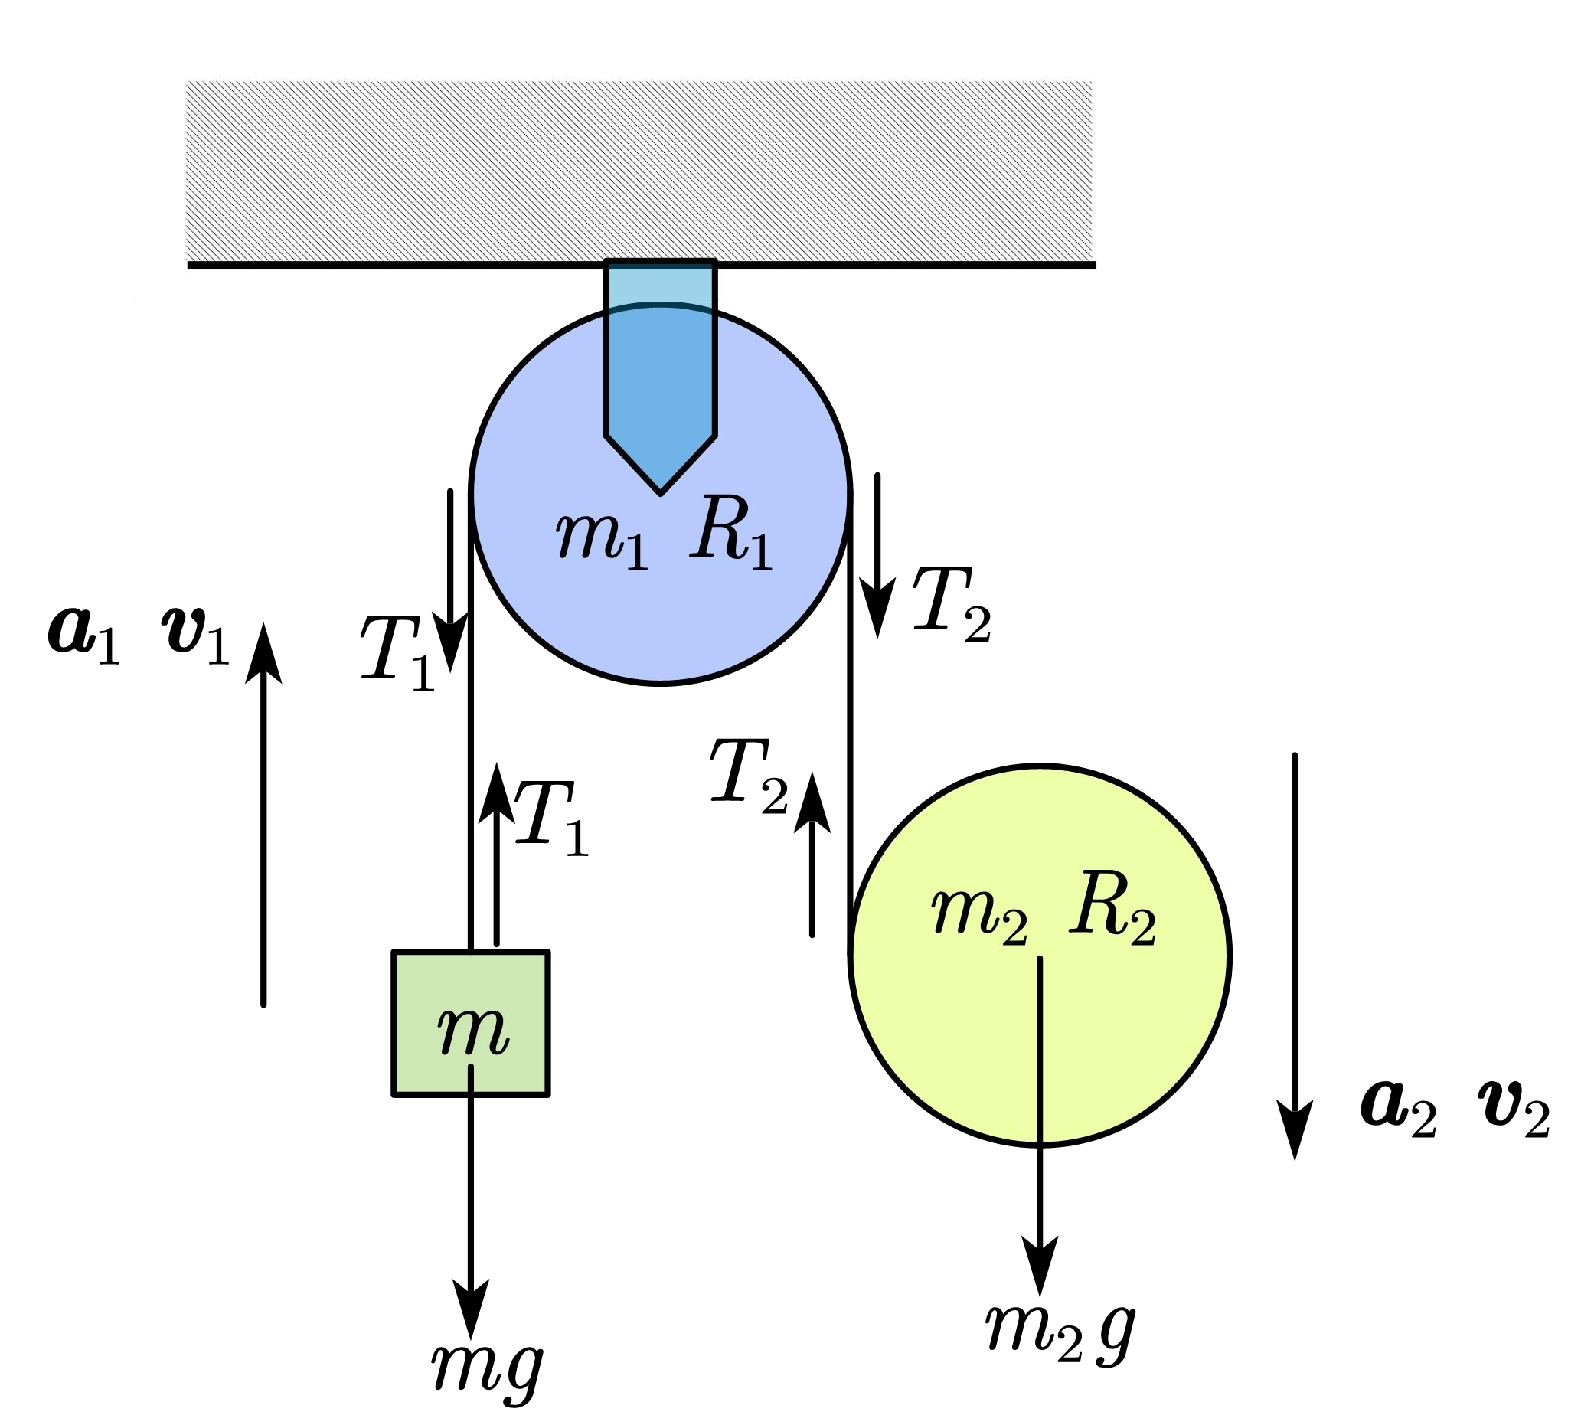
\includegraphics[width=0.7\linewidth]{6-22}
		\caption*{}
		\label{fig:6-22}
	\end{figure}
	\noindent According to the angular momentum theorem
	\begin{equation}
		\frac{\mathrm{d}L}{\mathrm{d}t}= =m_2g\left( R_1+R_2 \right) -mgR_1
	\end{equation}
	\begin{equation}
		L= mv_1R_1+m_2v_2\left( R_1+R_2 \right) +\frac{1}{2}m_1R_{1}^{2}\omega _1+\frac{1}{2}m_2R_{2}^{2}\omega _2 
	\end{equation}
	And there is no relative slip
	\begin{equation}
		R_1\omega_1=v_1
	\end{equation}
	\begin{equation}
		R_2\omega_2=v_2-v_1
	\end{equation}
	By combining these equations
	\begin{equation}
		mR_1a_1+m_2\left( R_1+R_2 \right) a_2+\frac{1}{2}m_1R_1a_1+\frac{1}{2}m_2R_2\left( a_2-a_1 \right) =m_2g\left( R_1+R_2 \right) -mgR_1
		\label{one}
	\end{equation}
	Study the rotation of the fixed pulley.
	\begin{equation}
		fR_1=\frac{1}{2}m_1R_1^2\beta_1=\frac{1}{2}m_1R_1^2\frac{a_1}{R_1}=\frac{1}{2}m_1R_1a_1
	\end{equation}
	Force analysis of disk and weight perspectively by isolation method, according to Newton's second law
	\begin{equation}
		m_2a_2=m_2g-T_2
	\end{equation}
	\begin{equation}
		T_1=T_2-f
	\end{equation}
	\begin{equation}
		ma_1=T_1-mg
	\end{equation}
	By combining these equations
	\begin{equation}
		m_2g-mg=ma_1+m_2a_2+\frac{1}{2}m_1a_1
		\label{two}
	\end{equation}
	By combining the (\ref{one}) and (\ref{two}) can we solve this problem.
	$$
	a_1=\frac{2(m_2-3m)}{6m+3m_1+m_2}g
	$$
	$$
	a_2=\frac{2(m+m_1+m_2)}{6m+3m_1+m_2}g
	$$
	Note that the $a_1$ can be both positive and negtive, if it is negetive, that means the direction of $a_1$ is opposite with the original suppose.
	\section{Question 6-25}
	Before reaching pure rolling, under the action of sliding friction, the center of mass of the ball accelerates and the speed slows down. According to the Newton's second law and the rotation law with the center of mass as the reference axis
	\begin{equation}
		ma=\mu mg\cos\theta-mg\sin\theta
	\end{equation}
	\begin{equation}
		\frac{2}{5}mr^2\beta=r\mu mg\cos\theta 
	\end{equation}
	Define $t$ as the time when ball reach pure rolling.
	\begin{equation}
		r(\omega_0-\beta t)=at
	\end{equation}
	According to kinematic formula
	\begin{equation}
		h_1=x_1\sin\theta=\frac{1}{2}at^2
	\end{equation}
	After reaching pure roll, the ball will roll and rise. According to conservation of mechanical energy
	\begin{equation}
		\frac{1}{2}m(at)^2+\frac{1}{2}\frac{2}{5}mr^2(\frac{at}{r})^2=mgh_2
	\end{equation}
	We can have
	$$
	h=h_1+h_2=\frac{2r^2\omega_0^2}{5g}\frac{\mu\cos\theta-\sin\theta}{7\mu\cos\theta-2\sin\theta}
	$$
	Note that there must be $\mu>\tan\theta$ or the ball can't move above because the fiction isn't enough.
	\section{Question 6-27}
	\subsection*{(1)}
	\subsubsection*{(i)}
	\noindent Since the direction of acceleration and angular acceleration is not determined, but will change with the adjustment of the parameters, it is best to take the right and clockwise as the positive direction, so that the positive and negative values can represent the direction.
	According to the Newton's second law and the rotation law with the middle axis as the reference axis.
	\begin{equation}
		ma=f-F\cos\theta
	\end{equation}
	\begin{equation}
		J\beta=Rf+rF
	\end{equation}
	And the pure rolling need
	\begin{equation}
		a=R\beta
		\label{pure}
	\end{equation}
	Combine (\ref{pure}) with others and kill the $f$ by liner calculate between equations.
	\begin{equation}
		(mR^2+J)a=R^2F\cos\theta-rRF
	\end{equation}
	The direction of $a$ is required to be negative.
	\begin{equation}
		a<0
	\end{equation}
	The solution is that
	\begin{equation}
		\theta>\arccos\frac{r}{R}
	\end{equation}
	\subsubsection*{(ii)}
	\noindent By solving  equations we get
	\begin{equation}
		f=-\frac{mrR+J\cos \theta}{mR^2+J}F<0
	\end{equation}
	The $f$ is always negtive, it means the direction of it is alwanys behind. Here is a restirction
	\begin{equation}
		|f|<\mu N=\mu(mg-F\sin\theta)
	\end{equation}
	The solution is that
	$$
	\mu \geqslant \frac{mrR+J\cos \theta}{mR^2+J}\frac{F}{\mu \left( mg-F\sin \theta \right)}
	$$
	\subsubsection*{(iii)}
	We can kill $f$ by liner calculate between equations. And to work out $a$.
	$$
	a=\frac{\left( R\cos \theta -r \right) RF}{mR^2+J}<0
	$$
	\section*{(2)}
	We know that the numerical value indicate the vector's direction so the anwsers above still correct\footnote{The $ \theta$ just take the opposite componet of (1).}.
	$$
	\theta<\arccos\frac{r}{R}
	$$
	$$
	\mu \geqslant \frac{mrR+J\cos \theta}{mR^2+J}\frac{F}{\mu \left( mg-F\sin \theta \right)}
	$$
	$$
	a=\frac{\left( R\cos \theta -r \right) RF}{mR^2+J}>0
	$$ 
	\section{Question 6-32}
	\subsection*{(1)}
	\noindent According to the momentum conservation law.
	\begin{equation}
		mv_0=mu_1+mu_2
	\end{equation}
	Because the collision is elastic and ignores friction, mechanical energy is conserved.
	\begin{equation}
		\frac{1}{2}mv_0^2=\frac{1}{2}mu_1^2+\frac{1}{2}mu_2^2
	\end{equation}
	Define $I_f$ as the impulse of friction from ground. According to the theorem of impulse and the angular momentum theorem, for ball-first we have
	\begin{equation}
		mv_1=mu_1+I_f
	\end{equation}
	\begin{equation}
		J\omega_1=J\omega_0-RI_f
	\end{equation}
	For ball-second we have
	\begin{equation}
		mv_2=mu_2-I_f
	\end{equation}
	\begin{equation}
		J\omega_2=RI_f
	\end{equation}
	Pure rolling requres
	\begin{equation}
		\omega_0=\frac{v_0}{R}
	\end{equation}
	\begin{equation}
		\omega_1=\frac{v_1}{R}
	\end{equation}
	\begin{equation}
		\omega_2=\frac{v_2}{R}
	\end{equation}
	So
	$$
	v_1=\frac{2}{7}v_0
	$$
	$$
	v_2=\frac{5}{7}v_0
	$$
	\subsection*{(2)}
	\noindent Calculate it directly.
	$$
	\Delta E_k=(\frac{1}{2}mv_0^2+\frac{1}{2}\frac{2}{5}m\omega_0^2)-(\frac{1}{2}mv_1^2+\frac{1}{2}\frac{2}{5}m\omega_1^2+\frac{1}{2}mv_2^2+\frac{1}{2}\frac{2}{5}m\omega_2^2)=\frac{2}{7}mv_0^2
	$$
	\section{Question 6-35}
	\begin{figure}[H]
		\centering
		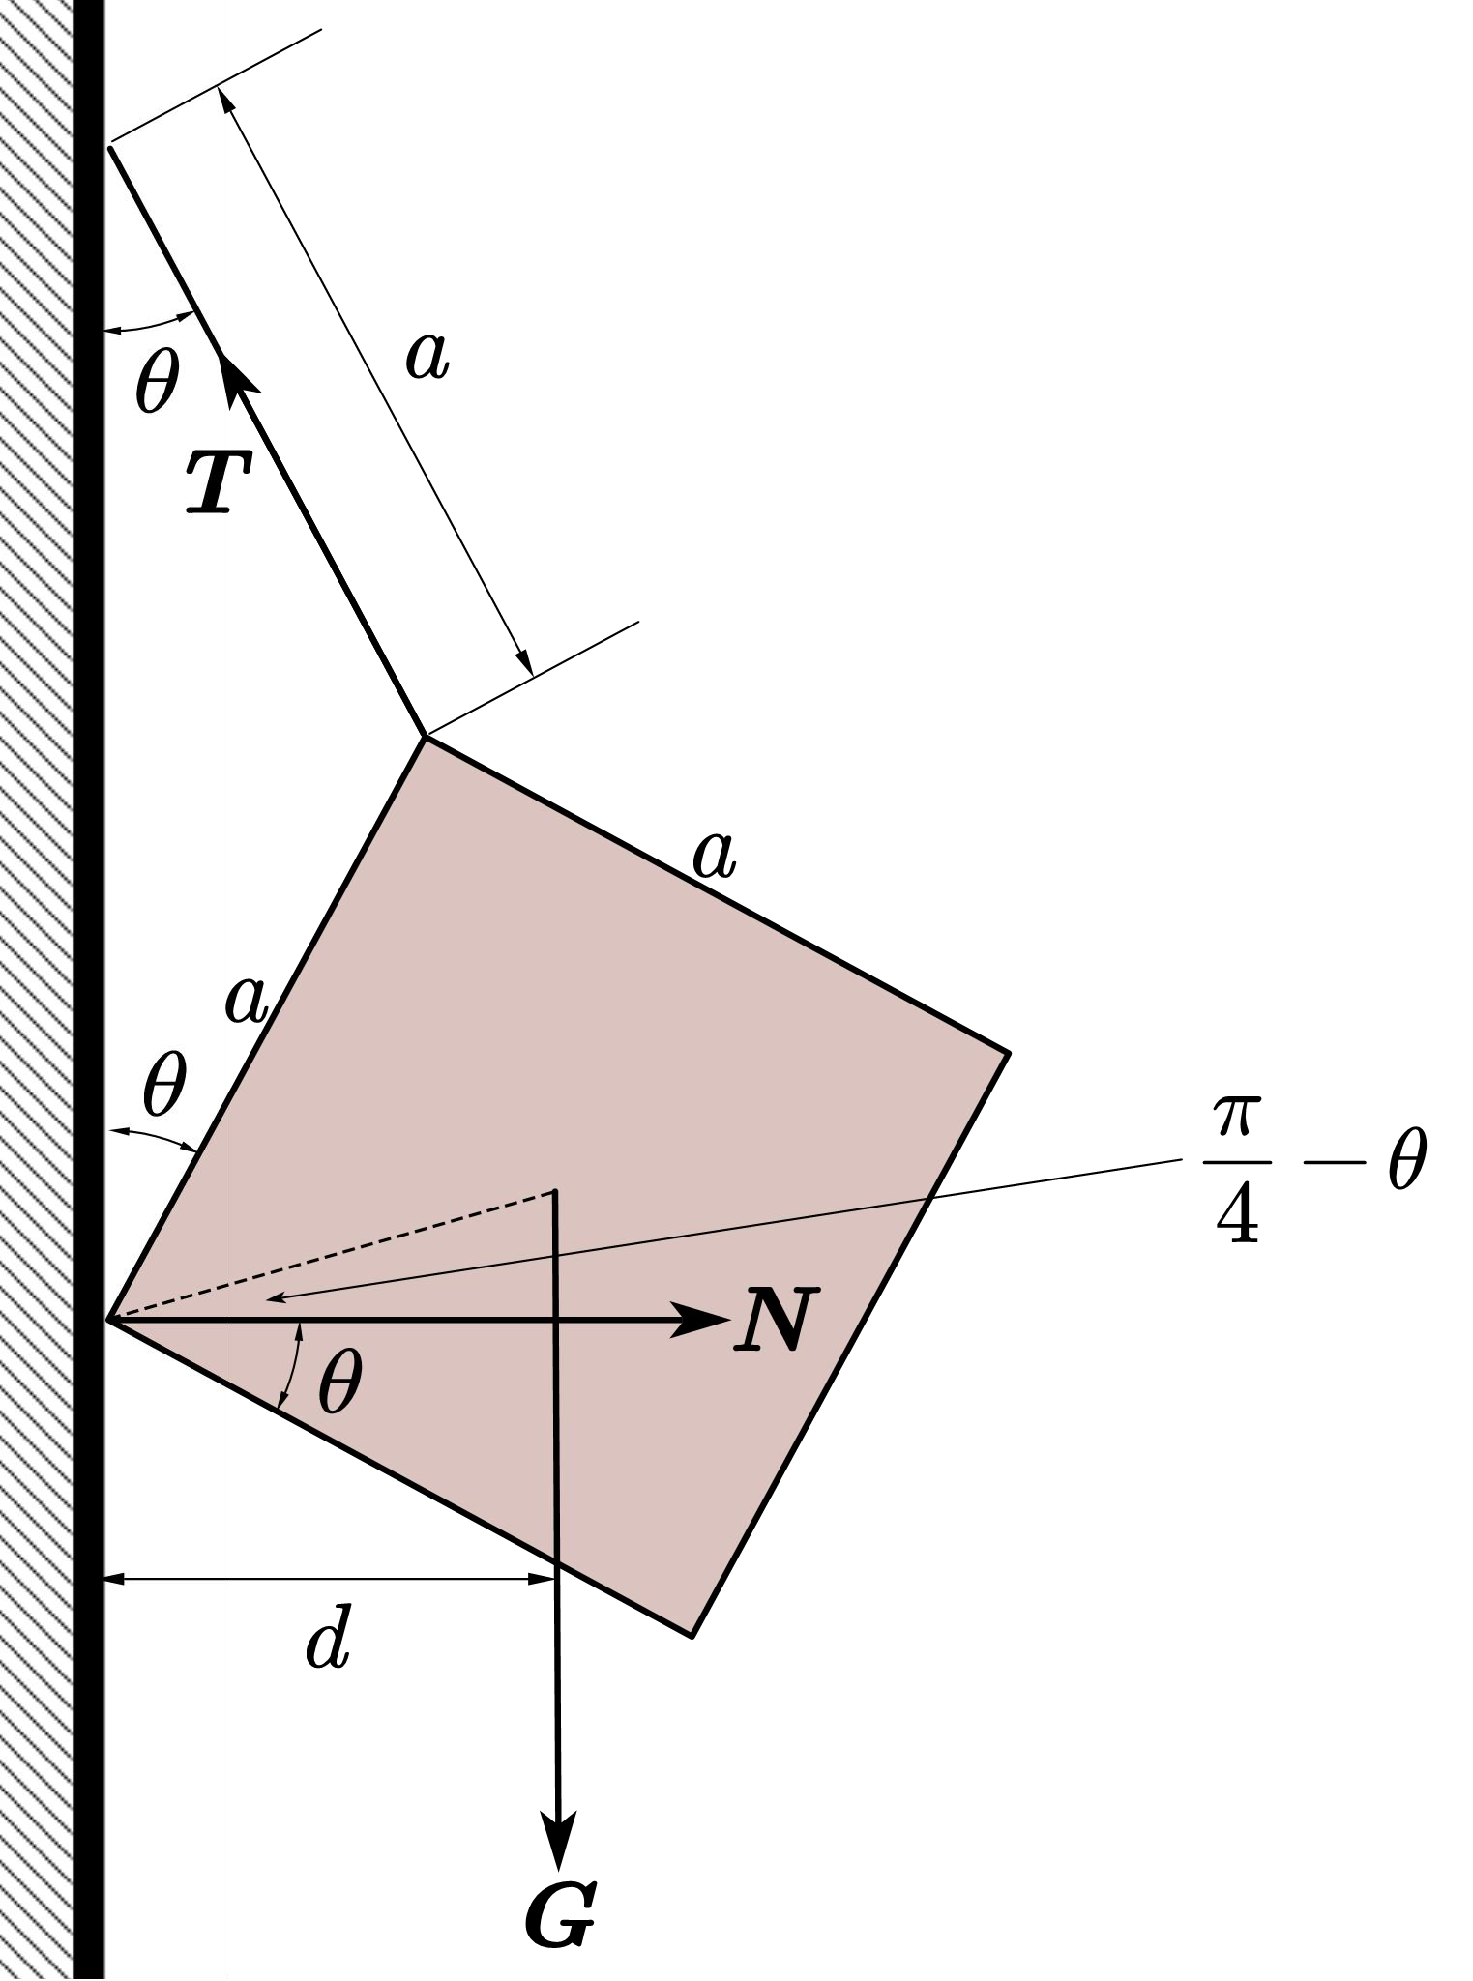
\includegraphics[width=0.7\linewidth]{6-35}
		\caption*{}
		\label{fig:6-35}
	\end{figure}
	\noindent According to the Mechanical equilibrium equation and some Geometric relation
	\begin{equation}
		mg=T\cos\theta
	\end{equation}
	\begin{equation}
		N=T\sin\theta
	\end{equation}
	\begin{equation}
		mg\frac{a}{\sqrt{2}}\cos(\frac{\pi}{4}-\theta)=N2a\cos\theta
	\end{equation}
	Easy to get
	$$
	T=\frac{\sqrt{10}}{3}mg
	$$
	\section{Question 6-40}
	\begin{figure}[H]
		\centering
		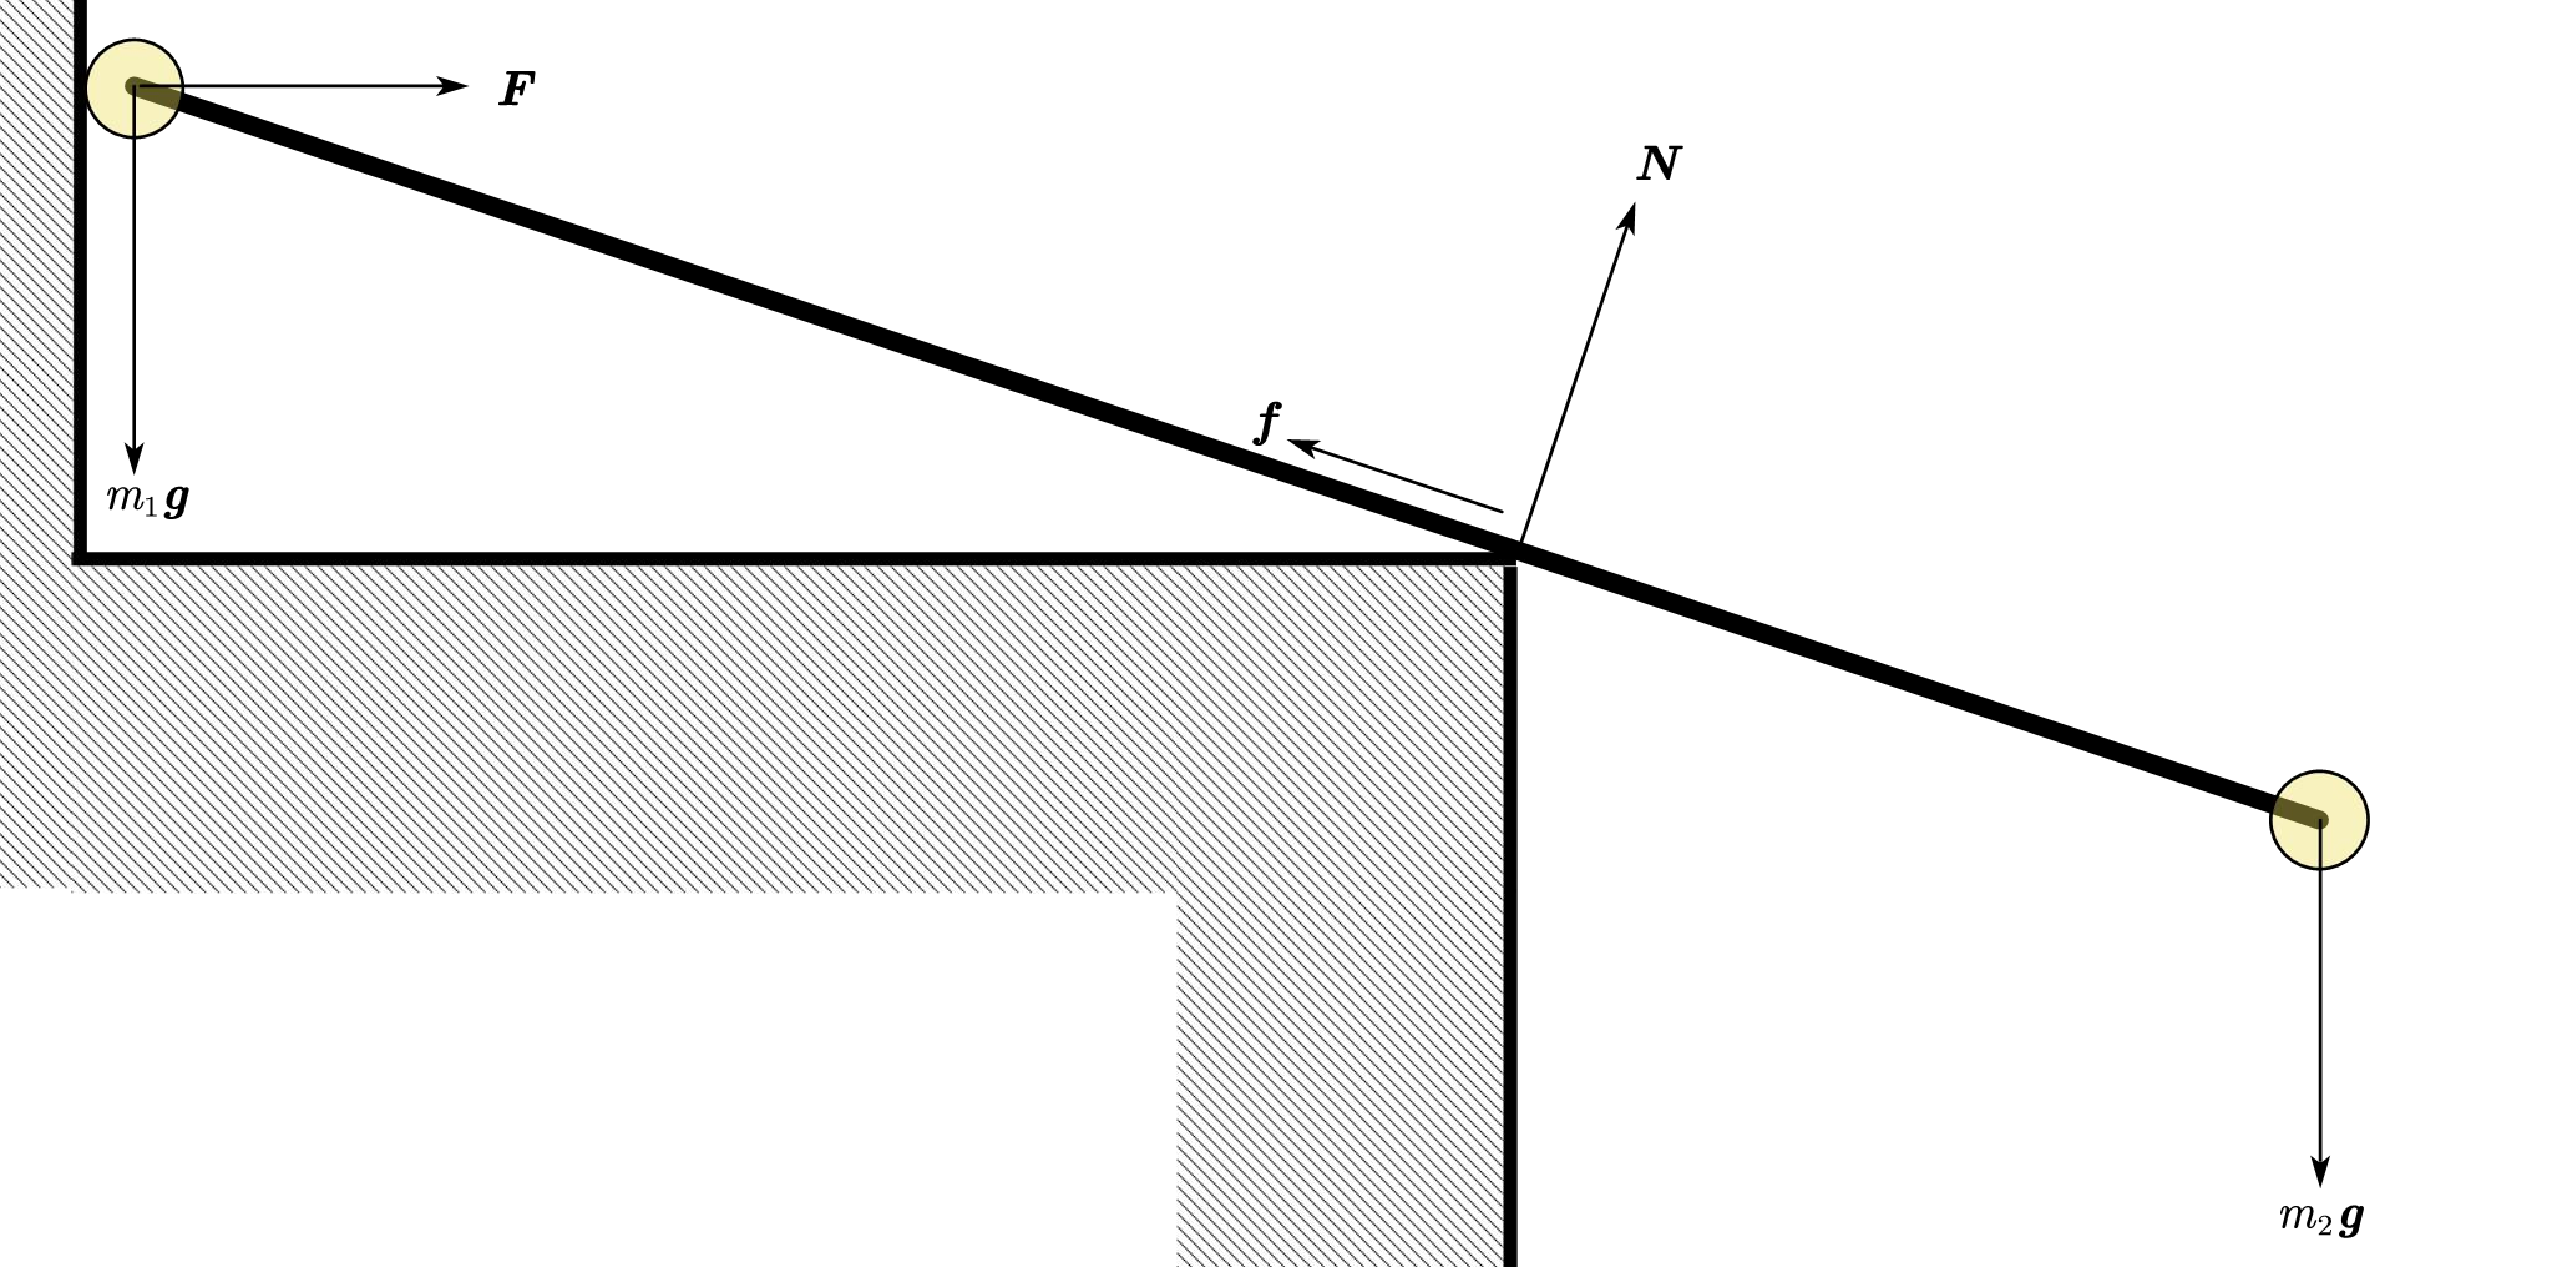
\includegraphics[width=0.9\linewidth]{6-40}
		\caption*{}
		\label{fig:6-40}
	\end{figure}
	\noindent According to the Mechanical equilibrium equation and the moment balance with the position of A as the reference point.
	\begin{equation}
		N\cos\theta+f\sin\theta=(m_1+m_2)g
	\end{equation}
	\begin{equation}
		f\cos\theta=F+N\sin\theta
	\end{equation}
	\begin{equation}
		N\frac{a}{\cos\theta}=m_2gl\cos\theta
		\label{MM}
	\end{equation}
	Take (\ref{MM}) into other equation
	\begin{equation}
		m_2g\frac{l}{a}\cos^3\theta+f\sin\theta=(m_1+m_2)g
		\label{YY}
	\end{equation}
	\begin{equation}
		f\cos\theta=F+m_2g\frac{l}{a}\sin\theta\cos^2\theta
	\end{equation}
	Consider $f\leqslant\mu N$, the (\ref{YY}) can be write like
	\begin{equation}
		(m_1+m_2)g\leqslant m_2g\frac{l}{a}\cos^3\theta+\mu m_2g\frac{l}{a}\cos^2\theta\sin\theta
	\end{equation}
	That is
	\begin{equation}
		1+\frac{m_1}{m_2}\leqslant\frac{l}{a}\cos^2\theta(\mu\sin\theta+\cos\theta)
	\end{equation}
	Considering the critical condition, the supporting force $\boldsymbol{F}$ of the left wall is 0.
	\begin{equation}
		1+\frac{m_1}{m_2}=\frac{l}{a}\cos\theta
	\end{equation}
	Obviously, $m_1$ is healvier than that case.
	\begin{equation}
		1+\frac{m_1}{m_2}\geqslant\frac{l}{a}\cos\theta
	\end{equation}
	As a result.
	\begin{equation}
			\frac{l}{a}\cos\theta\leqslant1+\frac{m_1}{m_2}\leqslant\frac{l}{a}\cos^2\theta(\mu\sin\theta+\cos\theta)
	\end{equation}

	However, the rightmost end of the inequality is not necessarily greater than or equal to the leftmost end, which requires the following.
	\begin{equation}
		\frac{l}{a}\cos\theta\leqslant\frac{l}{a}\cos^2\theta(\mu\sin\theta+\cos\theta)
	\end{equation}
	That is
	\begin{equation}
	\mu\geqslant\tan\theta
	\end{equation}
	So
	$$
	\frac{l}{a}\cos\theta\leqslant1+\frac{m_1}{m_2}\leqslant\frac{l}{a}\cos^2\theta(\mu\sin\theta+\cos\theta)\qquad\mu\geqslant\tan\theta
	$$
	\section{Question 6-45}
	\subsection*{(1)}
	\begin{figure}[H]
		\centering
		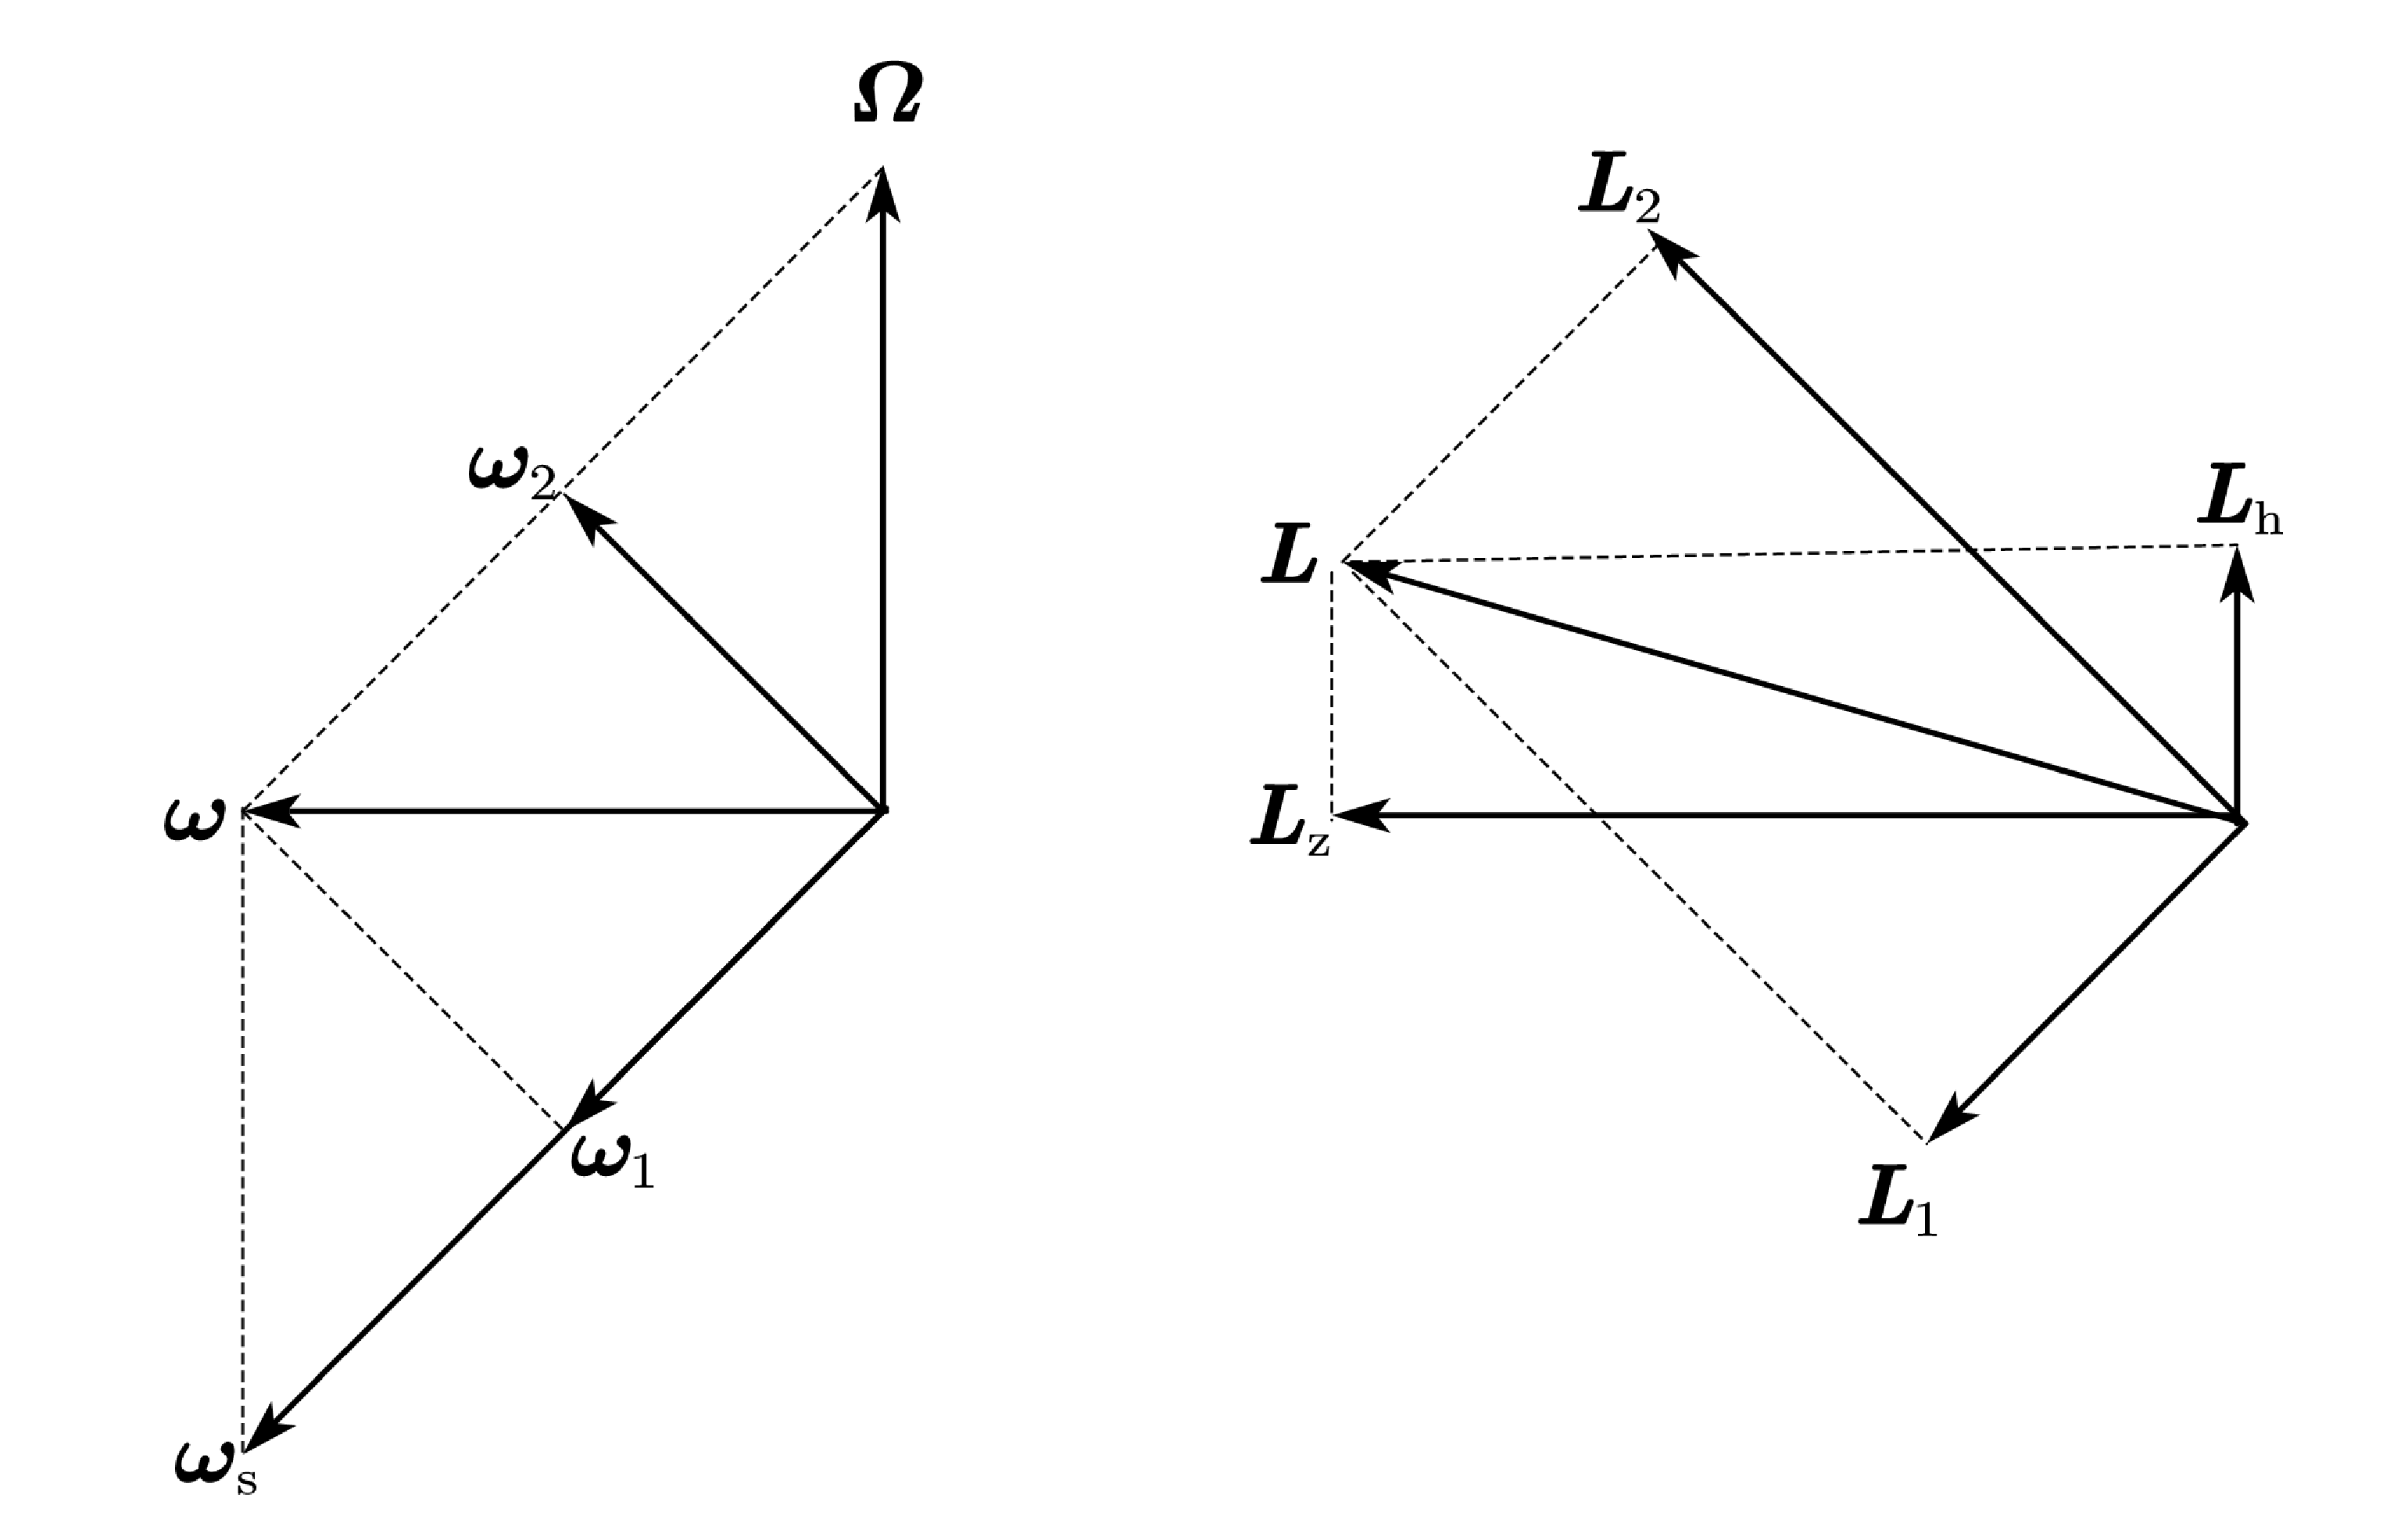
\includegraphics[width=0.7\linewidth]{6-45}
		\caption*{}
		\label{fig:6-45}
	\end{figure}
	\noindent As the figure, the instantaneous axis of rotation is the line between two points with instantaneous velocity of zero. That is, the line between two points of contact between a rigid body and the ground, it means the instantaneous axis of rotation is horizontal.
	
	\noindent Do geometric operations in vector drawings. The directions of $\boldsymbol{\omega_1}$ and $\boldsymbol{\omega_2}$ are the principal axis of inertia.
	\begin{equation}
		\omega_1=\omega_2=\frac{\varOmega}{\sqrt{2}}
	\end{equation}
	The principal axis of inertia makes the angular momentum and angular velocity go in the same direction.
	\begin{equation}
		L_1=J_1\omega_1
	\end{equation}
	\begin{equation}
		L_2=J_2\omega_2
	\end{equation}
	The moment of inertia can be obtained by the parallel axis theorem and the vertical axis theorem.
	\begin{equation}
		J_1=\frac{1}{2}mR^2
	\end{equation}
	\begin{equation}
		J_2=\frac{1}{2}J_1+mR^2
	\end{equation}
	Then the angular momentum is decomposed into the longitudinal and vertical instantaneous rotation directions.
	\begin{equation}
		L_{z}=\frac{L_1}{\sqrt{2}}+\frac{L_2}{\sqrt{2}}
	\end{equation}
	According to the nutation formula of rigid body.
	\begin{equation}
		\boldsymbol{M}=\boldsymbol{\varOmega}\times\boldsymbol{L}_{z}
	\end{equation}
	Write in scalar form
	\begin{equation}
		\sqrt{2}RF_{N}-\frac{\sqrt{2}}{2}Rmg=\frac{1}{\sqrt{2}}\varOmega L_{z}
	\end{equation}
	
	\noindent The solution is that
	$$
	F_{N}=\frac{7\sqrt{2}}{16}mR\varOmega^2+\frac{1}{2}mg
	$$
	\subsection*{(2)}
	\noindent Kinetic energy is examined on the principal axis of inertia.
	$$
	E_k=\frac{1}{2}J_1\omega_1^2+\frac{1}{2}J_2\omega_2^2=\frac{7}{16}mR^2\varOmega^2
	$$
\end{document}